\chapter{Approach}\label{chap:approach}

As stated in Section \ref{sec:goals}, the main objective of this thesis is to bring the Oghma framework to a web environment. This section describes the work plan for the project that will serve as the basis for the dissertation writing.

\section{Work Plan}\label{sec:work_plan}

The planning shown on Fig. \ref{fig:work_plan} was created based on the priorities of the tasks as well precedences between them. An initial study will be made regarding the Oghma framework, adaptive object-models architectures and the underlying design patterns that allow them to work, with an expected duration of four weeks. During that initial investigation, research will be performed regarding the best GUI patterns that allow end-users to modify the domain model for the application, with an expected duration of four weeks, bringing the total time for research and investigation to six weeks. During the final stages of initial research, the knowledge acquired is sufficient to start the development of the project which will serve as the basis for the dissertation report. The last phase of implementation will be coupled with tests and validation by external parties. Finally, the writing of the final dissertation report will be made throughout most of the planned process.

\begin{figure}[H]
  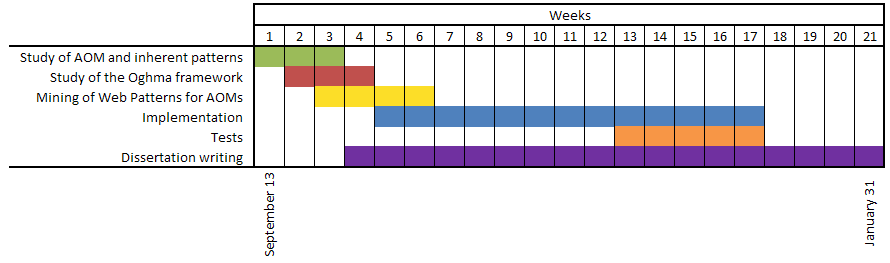
\includegraphics[width=\textwidth]{work_plan}
  \caption{Work plan for the duration of the thesis}
  \label{fig:work_plan}
\end{figure}

\section{Oghma and Design Patterns}\label{sec:oghma_and_design_patterns}

As the Oghma framework will act as the engine behind the interfaces to be developed, it is crucial that a solid knowledge of its API is acquired. Not only that, a careful study of the Oghma interface generation techniques must be performed in order to comprehend how the back end links itself with the user interfaces.

\section{Mining of Web Patterns for AOMs}\label{sec:mining_of_web_patterns}

This stage will be concerned with studying what the most effective GUI patterns are for applications of this type. A user should not perceive he or she is actually modifying the elementary structure of the system. As such, the user interface should be as intuitive as possible, with as less interference with the normal user workflow as possible. An initial study will be performed regarding current customization systems present in a multitude of websites --- what real-life paradigms and manipulation mechanisms are most commonly used, and try to transpose them to an AOM interface.

\section{Implementation}\label{sec:implementation}

Will all the acquired knowledge from stages \ref{sec:oghma_and_design_patterns} and \ref{sec:mining_of_web_patterns}, the implementation can now take place, alongside the final stages of mining of web patterns for AOMs. This stage will encompass the creation of a Ruby module for communicating with the Oghma framework, in order to use it as a back end for the system architecture. After this interface is complete, the initial GUIs will be created. These user interfaces will be static and prototypical in nature, in order to act as a blueprint from where the dynamic interfaces will be built. Finally, at the end of this stage, a proof-of-concept application will be created in order to validate the work developed during the past months.

Ruby was chosen mainly because of two factors: the familiarity with the language and the fact that the \textit{escolinhas.pt} platform is entirely written in Ruby, which will provide a much more seamless integration with the platform. The Oghma framework was chosen because it is the only one of its kind, as it was developed to be a reference framework for the construction of AOM systems.

A test-driven development (TDD) methodology will be used, in order to guarantee less bugs and a more consistent code base. This kind of development assumes failing tests are written \emph{before} the actual implementation --- defining a desired improvement or new function, producing code to pass that test and finally refactoring the new code to acceptable standards. This short cycle is repeated over and over again for every new feature (or group of features, if justifiable) to be implemented.

\section{Tasks}\label{sec:tasks}

This section will present a detailed list of all the major tasks planned for the next five months, as depicted in Table \ref{table:tasks}:

\begin{table}[H]
  \centering
  \begin{tabular}{c|c|c}
    \textbf{\textsc{Task Description}} & \textbf{\textsc{Starting Date}} & \textbf{\textsc{Planned Duration}}\\
    \hline
    \hline
    Oghma API study                                 & September 20, 2010  & 2 weeks\\\hline
    Oghma interface generation                      & October 4, 2010     & 2 weeks\\\hline
    Studying current paradigms of web customization & October 4, 2010     & 1.5 weeks\\\hline
    Adapting current paradigms to AOM interfaces    & October 13, 2010    & 2 weeks\\\hline
    Interfacing Oghma and Ruby                      & October 20, 2010    & 1 week\\\hline
    Initial interface building                      & October 27, 2010    & 2 weeks\\\hline
    Dynamic interfaces creation                     & November 15, 2010   & 4 weeks\\\hline
    Proof-of-concept application                    & December 13, 2010   & 3 weeks\\\hline
    Dissertation report writing                     & January 3, 2011     & 4 weeks\\\hline
    Article writing                                 & January 10, 2011    & 1.5 weeks\\\hline
  \end{tabular}
  \vspace{3mm}
  \caption{Detailed tasks descriptions and durations}
  \label{table:tasks}
\end{table}

It must be noted that, despite being presented as a four-week long task, the dissertation report writing will be performed throughout the duration of the thesis. The four weeks presented in Table~\ref{table:tasks} refer to the time that will be dedicated \emph{exclusively} to the writing.

